\section{N-dimensionales Punktdiagramm}

Falls man einen Datensatz darstellen will, der mehr als zwei unabhängige Variablen enthält, so kann die Darstellung in einem n-dimensionalen Punktdiagramm umgesetzt werden.

Datensätze in einem n-dimensionalen Merkmalsraum können in 2-dimensionalen Merkmalsräumen veranschaulicht werden und so gruppiert werden, dass eine Gesamtansicht auf die Daten möglich sind: In einer Scatterplot-Matrix \cite{viz}.

Als Versuchsdaten wurden Datensätze der World Bank \cite{worldbank} zur Bevölkerung, Arbeitsplätze und GDP der Schweiz im Verlauf der Zeit verwendet.

Ein n-dimensionales Punktdiagramm wurde im Test \texttt{dimensions} umgesetzt, sodass Datensätze mit der entsprechenden Konfigurationsdatei \texttt{meta.json} dargestellt werden können (Abbildung \ref{fig:nd}). Es wurde jedoch schnell erkannt, dass sich diese Art von Punktdiagramm nicht als interaktives Diagramm eignet:

\begin{itemize}
	\item Die Elemente der Scatterplot-Matrix hängen nicht zusammen. Die Achsen jedes Elements haben eine eigene Skalierung, darum ist die Umsetzung von Zoom, Tooltip, Detailanzeige so unmöglich.
	\item Ein weiterer Nachteil, der allerdings nicht mit der Interaktion zusammenhängt: Das Zustandekommen der einzelnen Scatterplots ist für den Benutzer nicht offensichtlich.
\end{itemize}

\begin{figure}[!htbp]
	\centering
	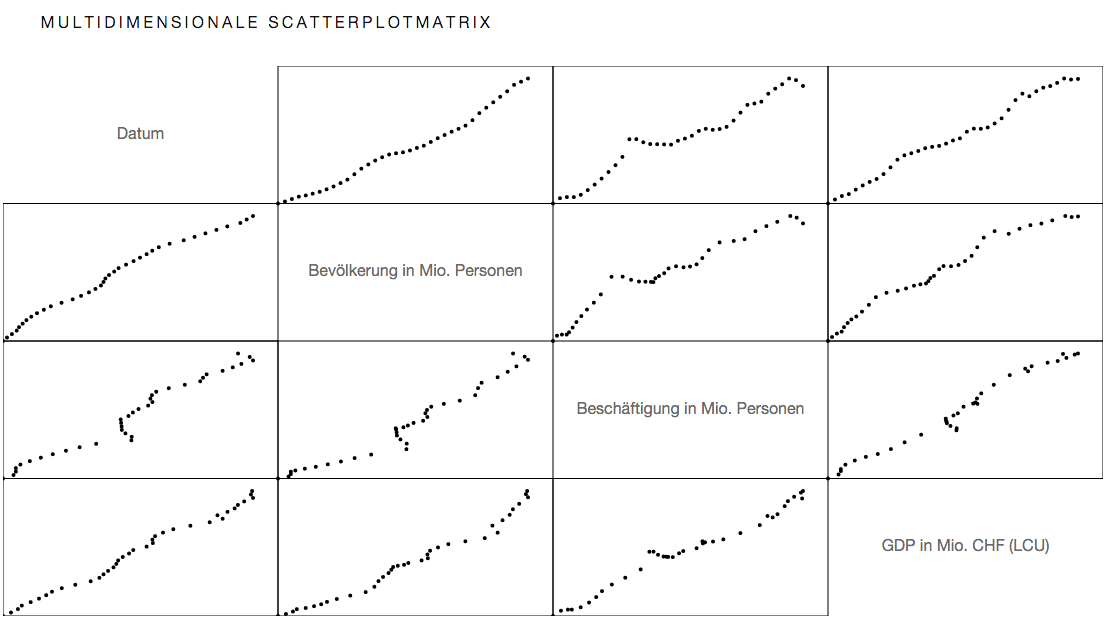
\includegraphics[width=\linewidth]{images/nd}
	\caption{Screenshot der Oberfläche der Applikation (n-dimensionales Punktdiagramm)}
	\label{fig:nd}
\end{figure}
